\section{Introduction}\label{s:intro}

\stress{Think before you write, be careful how you write, and take feedbacks
seriously}~\cite{Heiser-WebArticle2022}.


This section includes some motivations behind the work, explicitly or implicitly
highlights the research question, provides a high-level explanation of the
solution, and describes the contributions.

\textcolor{lightgray}{\lipsum[1]}

\parai{Makefile.}
%
It is typical to build a PDF from the \LaTeX{} sources using \texttt{make}, but
resist the temptation to fill the \texttt{Makefile} with complex and unnecessary
rules or recipes.
%
You only need one line, where you invoke \texttt{latexmk}.
%
This template should also come bundled with a \texttt{Makefile}, which should
suffice in virtually all scenarios.

\textcolor{lightgray}{\lipsum[3-4]}

\begin{figure}[tbh]
    %% The macro `\onecolgrid' is defined in `vusec.sty'
    %% NOTE: The suffix "./figs/" is implicitly included for this relative path.
    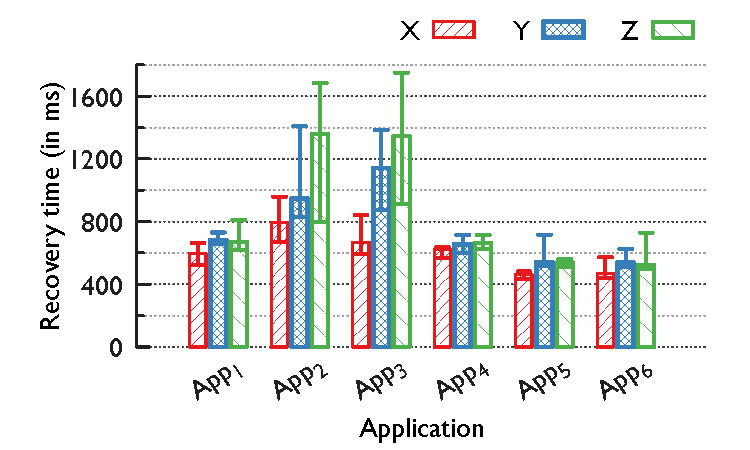
\includegraphics[width=\onecolgrid]{cache-by-app}
    %% Labels should immediately follow caption, to keep latex quiet.
    \figcap{Simple one-column figure. Please include a brief explanation or
    takeaway.}\label{fig:1col}
\end{figure}

\parai{Figures.}
%
Do not include figures that you do not refer to or discuss in the text.
%
Generate high-quality figures (Fig.~\ref{fig:1col})---think PDF or EPS.
%
With the number of tools and libraries that are available today for generating
beautiful plots, there is no excuse for producing ugly plots.
%
Figure caption must go at the bottom of a figure (Fig.~\ref{fig:3col}), and it
is also a good place to highlight the key takeaway of that figure.
%
Avoid using the position parameters `p' and `!', unless you are absolutely sure
that is exactly what you want.

\begin{figure*}[th]
    %% The macro `\threecolgrid' is defined in `vusec.sty'
    \begin{subfigure}[t]{\threecolgrid}
        %% NOTE: The suffix "./figs/" is implicitly included for these relative paths.
        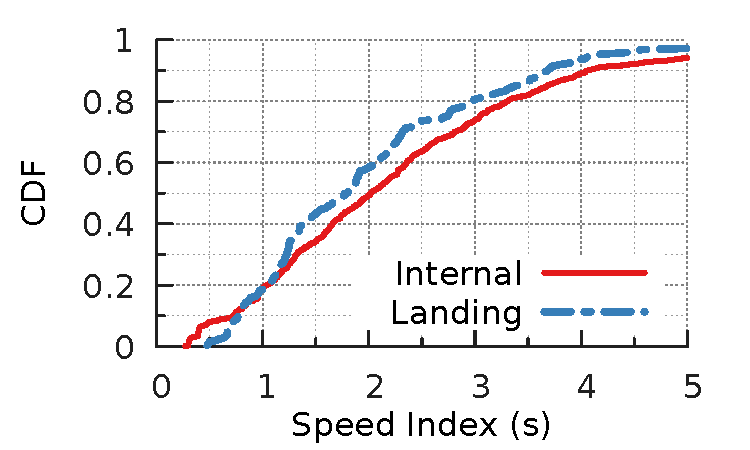
\includegraphics[width=\linewidth]{three-col/speed_index}
        \sfigcap{}\label{fig:3col-a}
    \end{subfigure}
    \begin{subfigure}[t]{\threecolgrid}
        %% NOTE: You do not have to mention the extension.
        %% (The example figures are in PDF format.)
        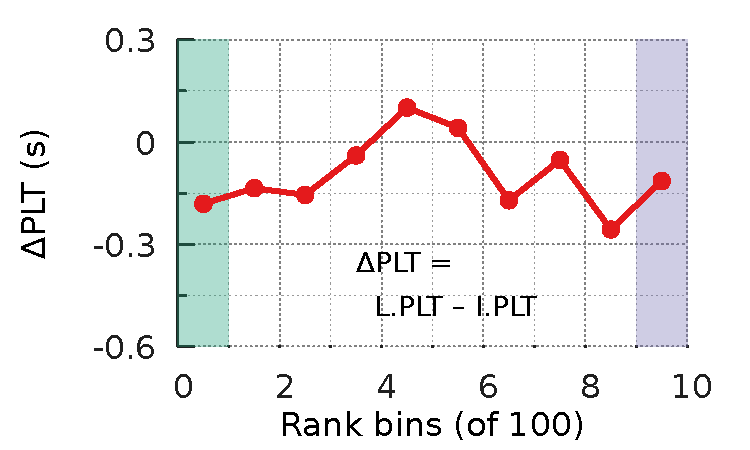
\includegraphics[width=\linewidth]{three-col/plt_ranks_diff}
        \sfigcap{}\label{fig:3col-b}
    \end{subfigure}
    \begin{subfigure}[t]{\threecolgrid}
        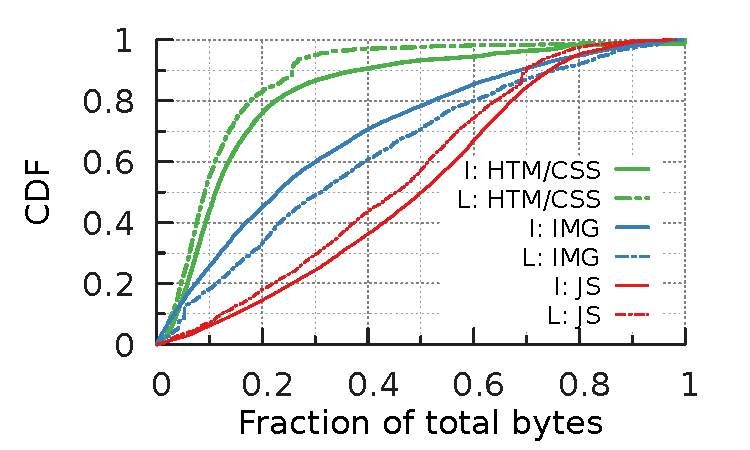
\includegraphics[width=\linewidth]{three-col/mimes}
        \sfigcap{}\label{fig:3col-c}
    \end{subfigure}
    %% Labels should immediately follow caption, to keep latex quiet.
    \figcap{Generate clear and beautiful figures (in PDF) that can be rendered side by side while still being easy to read and interpret. Choose colors wisely from the colorbrewer2.org website.}\label{fig:3col}
\end{figure*}

\textcolor{lightgray}{\lipsum[6-7]}

\begin{table}[tb]
    \centering
    \tabcap{A simple table describing the characteristics of a data set or the
    results of an experiment.}\label{tab:sample}
    \taburulecolor{black!45}
    \begin{tabu}{c|c|r|r|r|r}
        \toprule
        \multirow{2}{*}{\thead{Char.}} &
            \multirow{2}{*}{\thead{\#samples}} &
            \thead{Count} &
            \multicolumn{3}{c}{\thead{Perf. Score}}\\
        &
            &
            \thead{of items} &
            \thead{X} & \thead{Y} & \thead{Z} \\
        \midrule
        \stress{P}
            & 214 & 56 & 9 & 23 & 24 \\
        \stress{Q}
            & 117 & 27 & 7 & 10 & 10 \\
        \stress{R}
            & 222 & 11 & 6 & 4 & 1 \\
        \stress{S}
            & 187 &  9 & 1 & 6 & 2 \\
        \stress{T}
            & 180 & 16 & 7 & 5 & 4 \\
        \bottomrule
    \end{tabu}

\end{table}

\parai{Tables.}
%
The caption must go at the top of the table (Tab.~\ref{tab:sample}).
%
Do not use \texttt{\textbackslash{}hrule}.
%
Use \texttt{\textbackslash{}toprule} above the heading,
\texttt{\textbackslash{}midrule} below the heading, and
\texttt{\textbackslash{}bottomrule} below the last row.
%
You could also use \texttt{\textbackslash{}hrule} as a row separator.
%
Right align numerical values, and use math-mode for (large) numerical values to
force \LaTeX{} to use monospaced fonts and ensure right-alignment functions as
expected.

\textcolor{lightgray}{\lipsum[12-14]}

We summarize our contributions as follows.

\case{}
%
\textcolor{lightgray}{\lipsum[10][2-4]}

\case{}
% 
\textcolor{lightgray}{\lipsum[11][4-8]}

\case{}
% 
\textcolor{lightgray}{\lipsum[12][2-6]}

\case{}
% 
\textcolor{lightgray}{\lipsum[16][4-8]}

Depending on your degree program and/or supervisor, you may need to furnish the
“Artifact Appendix” (\S\ref{s:appendix}).


%%% Local Variables:
%%% mode: latex
%%% TeX-master: "../thesis"
%%% End:
